\appendix

\chapter{Appendix}

\section{Relationship between \acl{MAC} Operations and the Number of Parameters}\label{sec:appendix:macs}

For a convolution operation, the number of parameters of a layer is not
representative of its computational complexity. Each kernel has to be spatially
convolved with the entire input. The resulting convolutional complexity is, for
one part, highly dependent on the input size, and for the other part, higher
than the number of parameters.\\

Without loss of generality, consider a 2D square matrix $M$ of size $m \times
m$, and a 2D convolution kernel $K$ of size $k \times k$, with $k\ll m$. The output
of the spatial convolution of $M$ by $K$ is denoted $O$. The matrix $O$ is of
size $(m-k+1) \times (m-k+1)$. Each one of the $(m-k+1)^2$ elements of $O$
necessitates $k^2$ multiplications and $k^2-1$ additions. For the sake of
simplicity, we will consider $k^2$ \acfp{MAC} operations per element of $O$. The
total number of \acp{MAC} needed to compute $O$, denoted $\mu$, is therefore:\\
$$
    \mu = (m-k+1)^2 \times k^2
$$\\

Considering that there are $k^2$ elements in $K$, the ratio between the number
of \acp{MAC} and the number of parameters is:

$$
    \frac{\mu}{k^2} = (m-k+1)^2
$$\\


Since $k\ll m$, the ratio $\frac{\mu}{k^2}$ is always greater than $1$, and
grows quadratically with $m$. Therefore, for a 2D convolution, the computational
complexity can roughly be estimated as $(m-k+1)^2$ times the number of
parameters in the convolution kernel.\\

\section{Scheduling of the Mixing Coefficient \texorpdfstring{$\lambda$}{lambda}}
\label{sec:appendix:annihilation}

This section presents the test accuracy of a Conv4 network trained on CIFAR-10
with the method introduced in \cref{sec:chap1:weight_reparam} when scheduling is
applied on the mixing coefficient $\lambda$. Two trends are tested for
$\lambda$: increasing and decreasing. Given a $\lambda_\text{max}$, a maximum
number of epochs $e_\text{max}$, the current epoch $e$, and a shape parameter
$p$, the decreasing scheduling is defined as follows:\\
$$
    \lambda_e = \lambda_\text{max}  \sqrt[p~]{1 - \displaystyle\left(\frac{e}{e_\text{max}}\right)^p}
$$\\
and the increasing scheduling is defined as follows:\\
$$\\
    \lambda_e = \lambda_\text{max} \left( 1- \sqrt[p~]{ 1 - \left(\frac{e}{e_\text{max}}\right)^p} \right)
$$\\
Examples of the evolution of $\lambda$ for different values of $p$ are shown in
\cref{fig:appendix:annihiliation_inc_dec} and the related performances in
\cref{sec:appendix:annihiliation_table}.\\

\begin{table}[htbp]
    \centering
    \begin{tabular}{lllc}
        \toprule
        \textbf{pruning rate} (\%) & \textbf{$\lambda$ Trend} & $p$             & \textbf{Test Accuracy} (\%) \\
        \midrule
        \multirow{6}{*}{90}        & \multirow{3}{*}{incr.}   & 0.6             & 85.46 $\pm$ 0.18            \\
                                   &                          & 1               & 85.43 $\pm$ 0.46            \\
                                   &                          & $\frac{1}{0.6}$ & 84.96 $\pm$ 0.53            \\
        \cline{2-4}
                                   & \multirow{3}{*}{decr.}   & 0.6             & 85.36 $\pm$ 0.59            \\
                                   &                          & 1               & 85.55 $\pm$ 0.47            \\
                                   &                          & $\frac{1}{0.6}$ & 85.50 $\pm$ 0.29            \\
        \midrule
        \multirow{6}{*}{95}        & \multirow{3}{*}{incr.}   & 0.6             & 84.00 $\pm$ 0.85            \\
                                   &                          & 1               & 79.28 $\pm$ 0.96            \\
                                   &                          & $\frac{1}{0.6}$ & 66.43 $\pm$ 05.13           \\
        \cline{2-4}
                                   & \multirow{3}{*}{decr.}   & 0.6             & 83.53 $\pm$ 0.65            \\
                                   &                          & 1               & 83.42 $\pm$ 0.50            \\
                                   &                          & $\frac{1}{0.6}$ & 84.07 $\pm$ 0.92            \\
        \midrule
        \multirow{6}{*}{99}        & \multirow{3}{*}{incr.}   & 0.6             & 14.27 $\pm$ 3.21            \\
                                   &                          & 1               & 11.05 $\pm$ 01.26           \\
                                   &                          & $\frac{1}{0.6}$ & 10.33 $\pm$ 0.43            \\
        \cline{2-4}
                                   & \multirow{3}{*}{decr.}   & 0.6             & 34.36 $\pm$ 33.40           \\
                                   &                          & 1               & 52.51 $\pm$ 29.65           \\
                                   &                          & $\frac{1}{0.6}$ & 45.37 $\pm$ 32.32           \\
        \bottomrule
    \end{tabular}
    \caption{Conv4 test accuracy on CIFAR-10, with $\lambda=50$, for increasing
        (\emph{incr.}) and decreasing (\emph{decr.}) scheduling for various pruning
        rates and values of the parameter $p$. The networks have been trained for
        300 epochs.}
    \label{sec:appendix:annihiliation_table}
\end{table}


\begin{figure}[!h]
    \centering
    \subfloat[Increasing scheduling\label{fig:appendix:annihilation_increasing}]{
        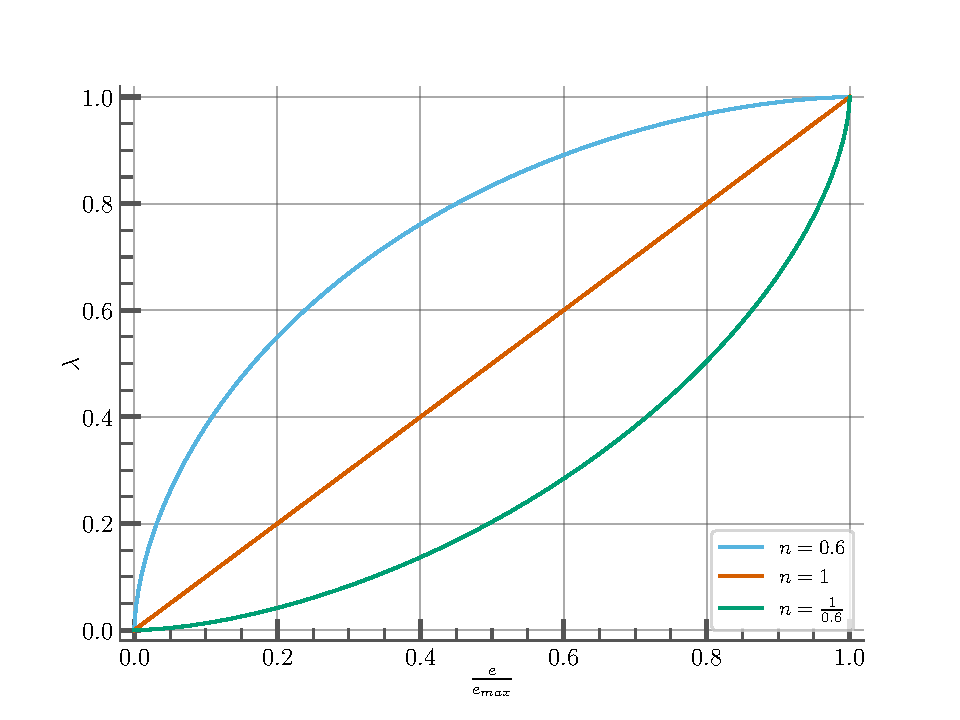
\includegraphics[width=0.49\textwidth]{appendix/assets/annihiling_lambda_max.pdf}}
    \subfloat[Decreasing
        scheduling\label{fig:appendix:annihilation_decreasing}]{
        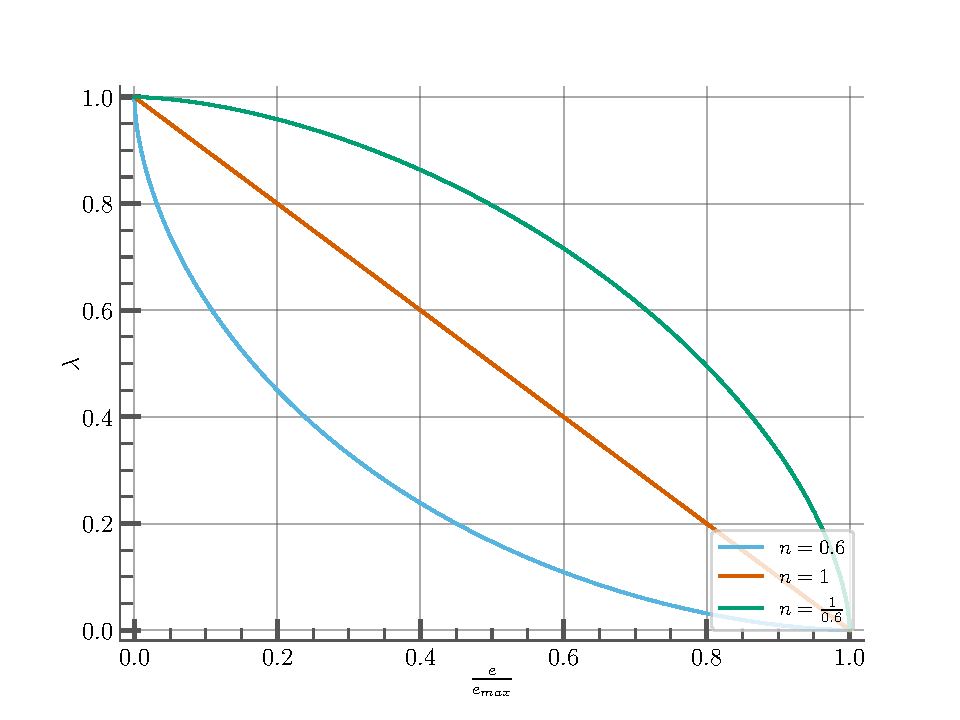
\includegraphics[width=0.49\textwidth]{appendix/assets/annihiling_lambda_min.pdf}}
    \caption{Evolution of the mixing coefficient $\lambda$ for different values
        of $p$ and for increasing and decreasing scheduling. Best viewed in color.}
    \label{fig:appendix:annihiliation_inc_dec}
\end{figure}

\section{Xavier and Kaiming Initialisations}
\label{sec:appendix:xavier_init}
Glorot and Kaiming initializations are strategies for initializing the weights
of neural networks. They are designed to help mitigate the issues of vanishing
and exploding gradients, which can occur during the training of deep neural
networks.\\

Glorot Initialization, also known as Xavier Initialization, suggests that the
initial weights of the network should be drawn from a distribution with zero
mean and a specific variance. The variance is dependent on the number of input
and output neurons in the weight tensor. Kaiming initialisation is a
modification of Glorot initialisation that is tailored for neural networks with
ReLU activations. It is designed to take into account the fact that ReLU
activations nullify half of the input values. These two types of initialisation
can be used with either a normal or uniform distribution. They impact the
standard deviation (and consequently the variance) of the underlying
distribution. The standard deviation for Glorot normal initialisation is
computed as follows:\\

\begin{equation}
    \sigma = \sqrt{\frac{2}{n_\text{in} + n_\text{out}}}
\end{equation}\\

where $n_\text{in}$ and $n_\text{out}$ are the number of input and output
neurons in the weight tensor. The standard deviation for Kaiming normal
initialisation is computed as follows:\\

\begin{equation}
    \sigma = \frac{1}{\sqrt{n_\text{in}}}
\end{equation}

where $n_\text{in}$ is the number of input neurons in the weight tensor.\\

It is important to note that, when using the Pytorch framework, this standard
deviation is adapted depending on the type of non-linearities used in the
network. For instance, using \ac{ReLU} activation functions require multiplying
the standard deviation by $\sqrt{2}$ \cite{pytorch_init}.\\